\element{liaisons statique}{
\begin{questionmult}{liaisonstat 00}
Soit le torseur des actions mécaniques suivant : 
$\torseurl{X_O\vx{}+Y_O\vy{}+Z_O\vz{}}{L_O\vx{}+M_O\vy{}+N_O\vz{}}{O}$.

%\begin{center}
%%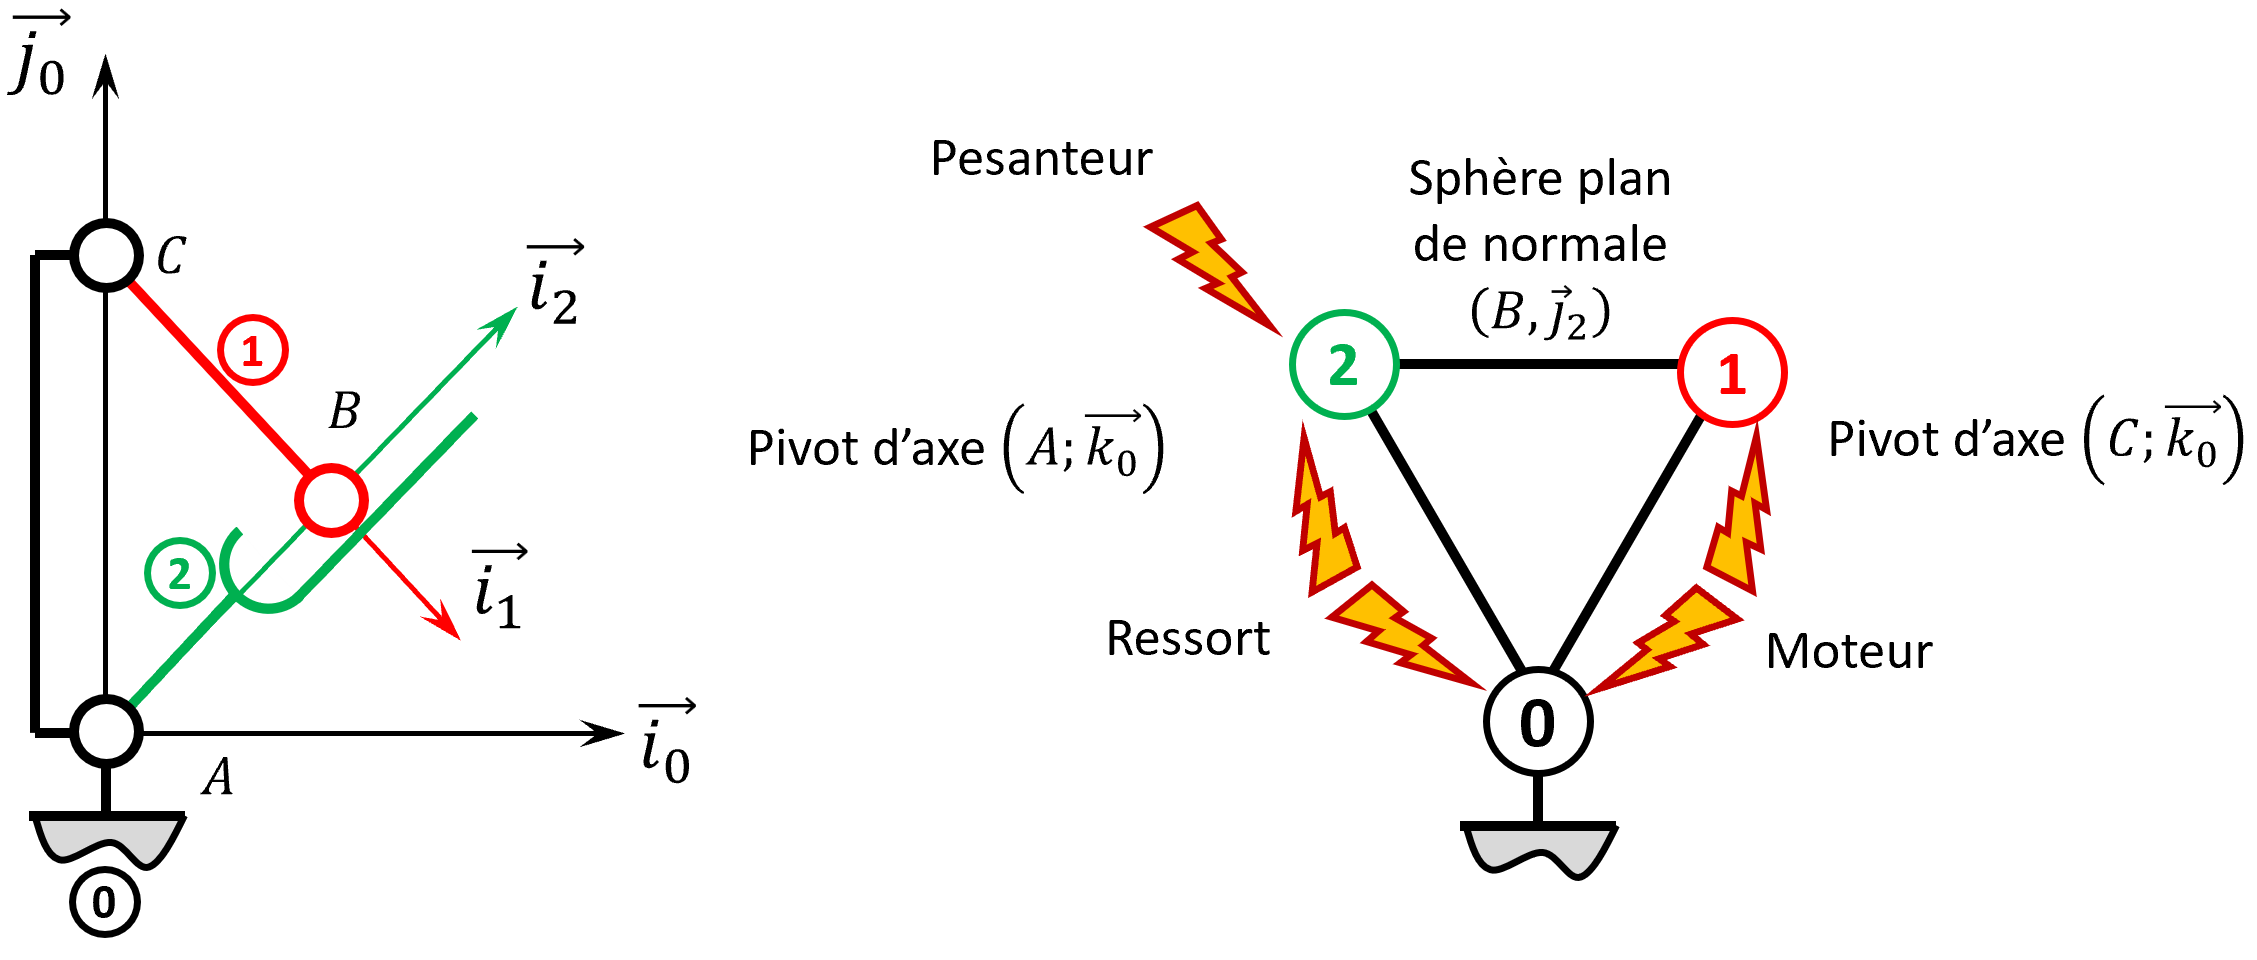
\includegraphics[width=.95\linewidth]{pfs_strategie_sympact_01}
%\end{center}
	\begin{reponses}
	\mauvaise{Ponctuelle}
	\mauvaise{Sphère plan}
	\mauvaise{Linéaire annulaire}
	\mauvaise{Sphère cylindre}
	\mauvaise{Linéaire rectiligne}
	\mauvaise{Cylindre plan}
	\mauvaise{Rotule}
	\mauvaise{Sphérique}
	\mauvaise{Rotule à doigt}
	\mauvaise{Pivot glissant}
	\mauvaise{Pivot}
	\mauvaise{Glissière}
	\mauvaise{Hélicoïdale}
	\bonne{Encastrement}
	\mauvaise{d'axe}
	\mauvaise{de normale}
	\mauvaise{de centre}
	\mauvaise{de direction}
	\mauvaise{$O$}
	\mauvaise{$\overrightarrow{x}$}
	\mauvaise{$\overrightarrow{y}$}
          \mauvaise{$\overrightarrow{z}$}
	\end{reponses}
\end{questionmult}
\\}

\element{liaisons statique}{
\begin{questionmult}{liaisonstat 01}
Soit le torseur des actions mécaniques suivant : 
$\torseurl{X_O\vx{}}{\vect{0}}{O}$.
%\begin{center}
%%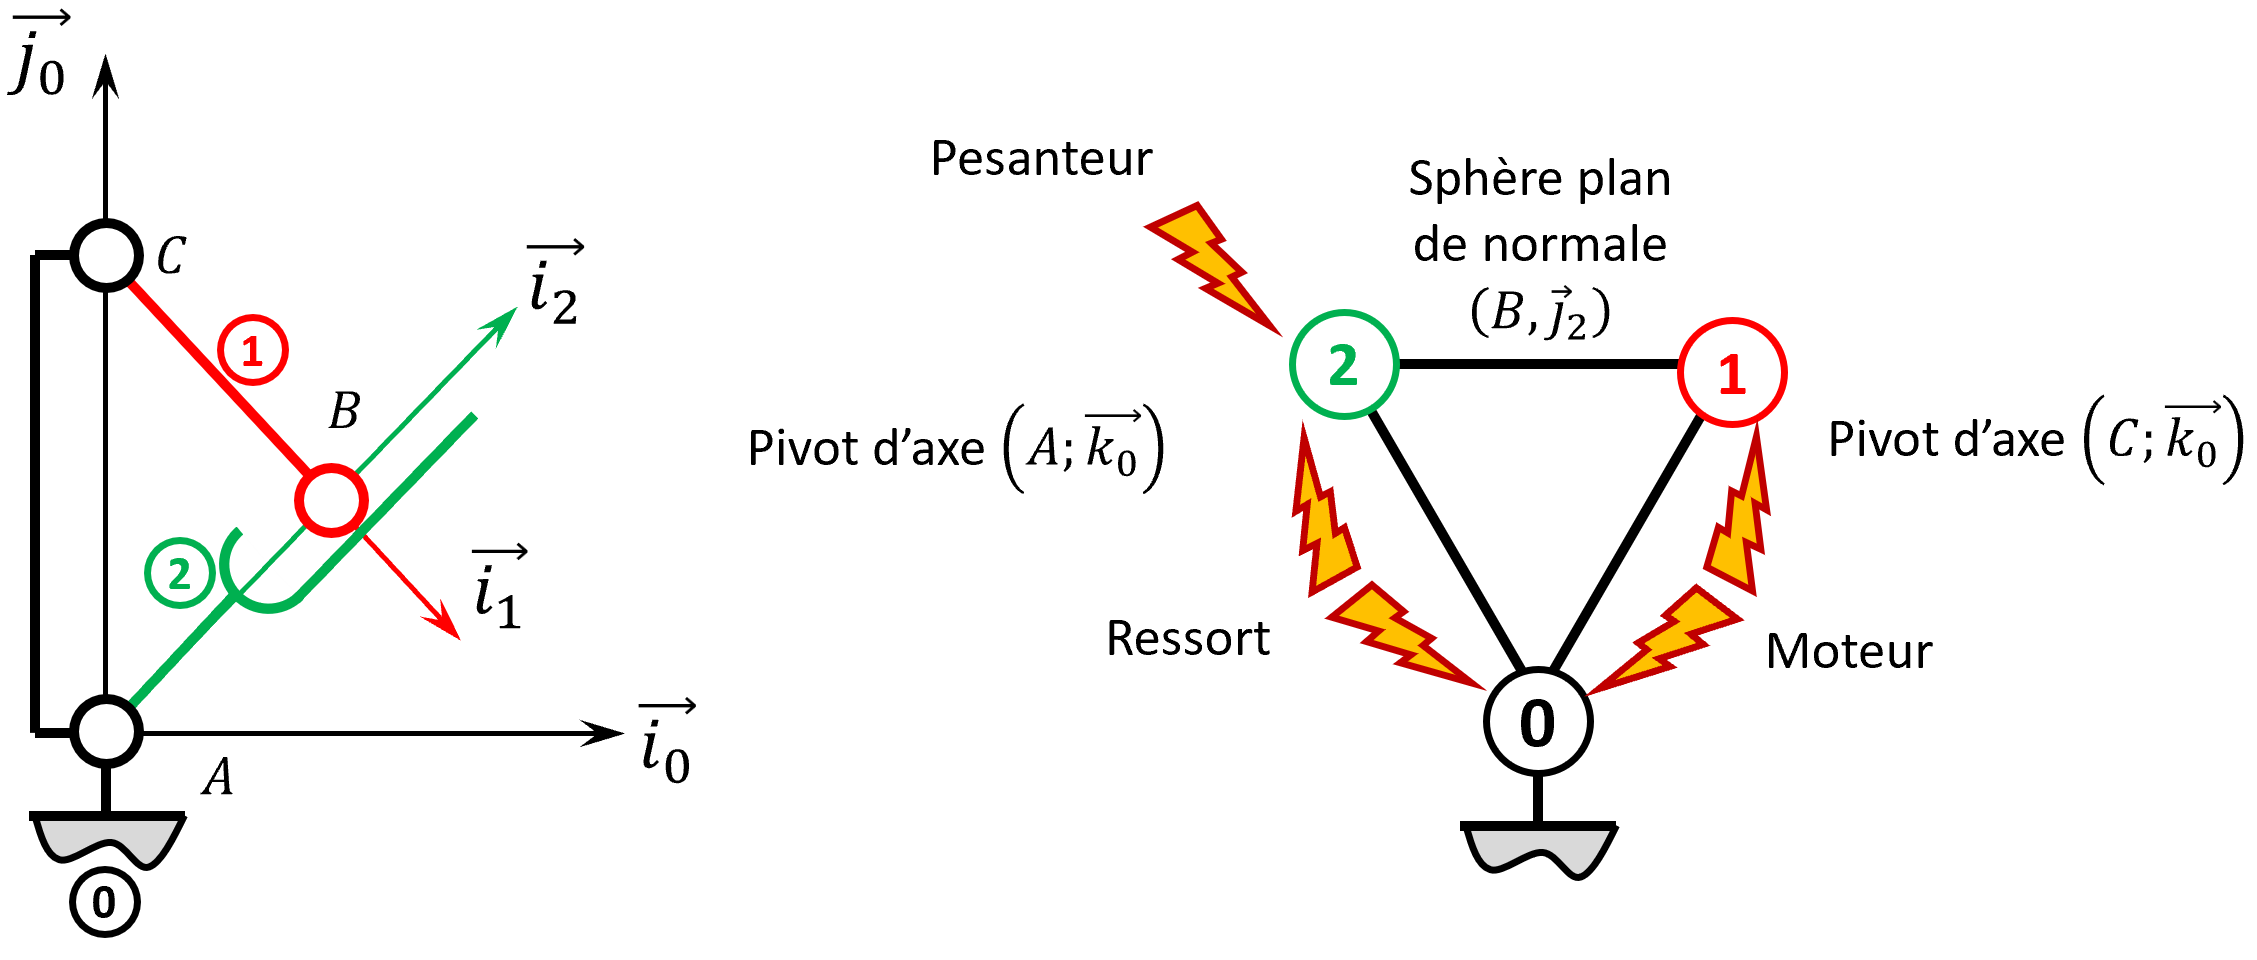
\includegraphics[width=.95\linewidth]{pfs_strategie_sympact_01}
%\end{center}
	\begin{reponses}
	\bonne{Ponctuelle}
	\bonne{Sphère plan}
	\mauvaise{Linéaire annulaire}
	\mauvaise{Sphère cylindre}
	\mauvaise{Linéaire rectiligne}
	\mauvaise{Cylindre plan}
	\mauvaise{Rotule}
	\mauvaise{Sphérique}
	\mauvaise{Rotule à doigt}
	\mauvaise{Pivot glissant}
	\mauvaise{Pivot}
	\mauvaise{Glissière}
	\mauvaise{Hélicoïdale}
	\mauvaise{Encastrement}
	\mauvaise{d'axe}
	\bonne{de normale}
	\mauvaise{de direction}
	\mauvaise{de centre}
	\mauvaise{$O$}
	\bonne{$\overrightarrow{x}$}
	\mauvaise{$\overrightarrow{y}$}
          \mauvaise{$\overrightarrow{z}$}
	\end{reponses}
\end{questionmult}
\\}

\element{liaisons statique}{
\begin{questionmult}{liaisonstat 02}
Soit le torseur des actions mécaniques suivant : 
$\torseurl{Y_O\vy{}}{\vect{0}}{O}$.
%\begin{center}
%%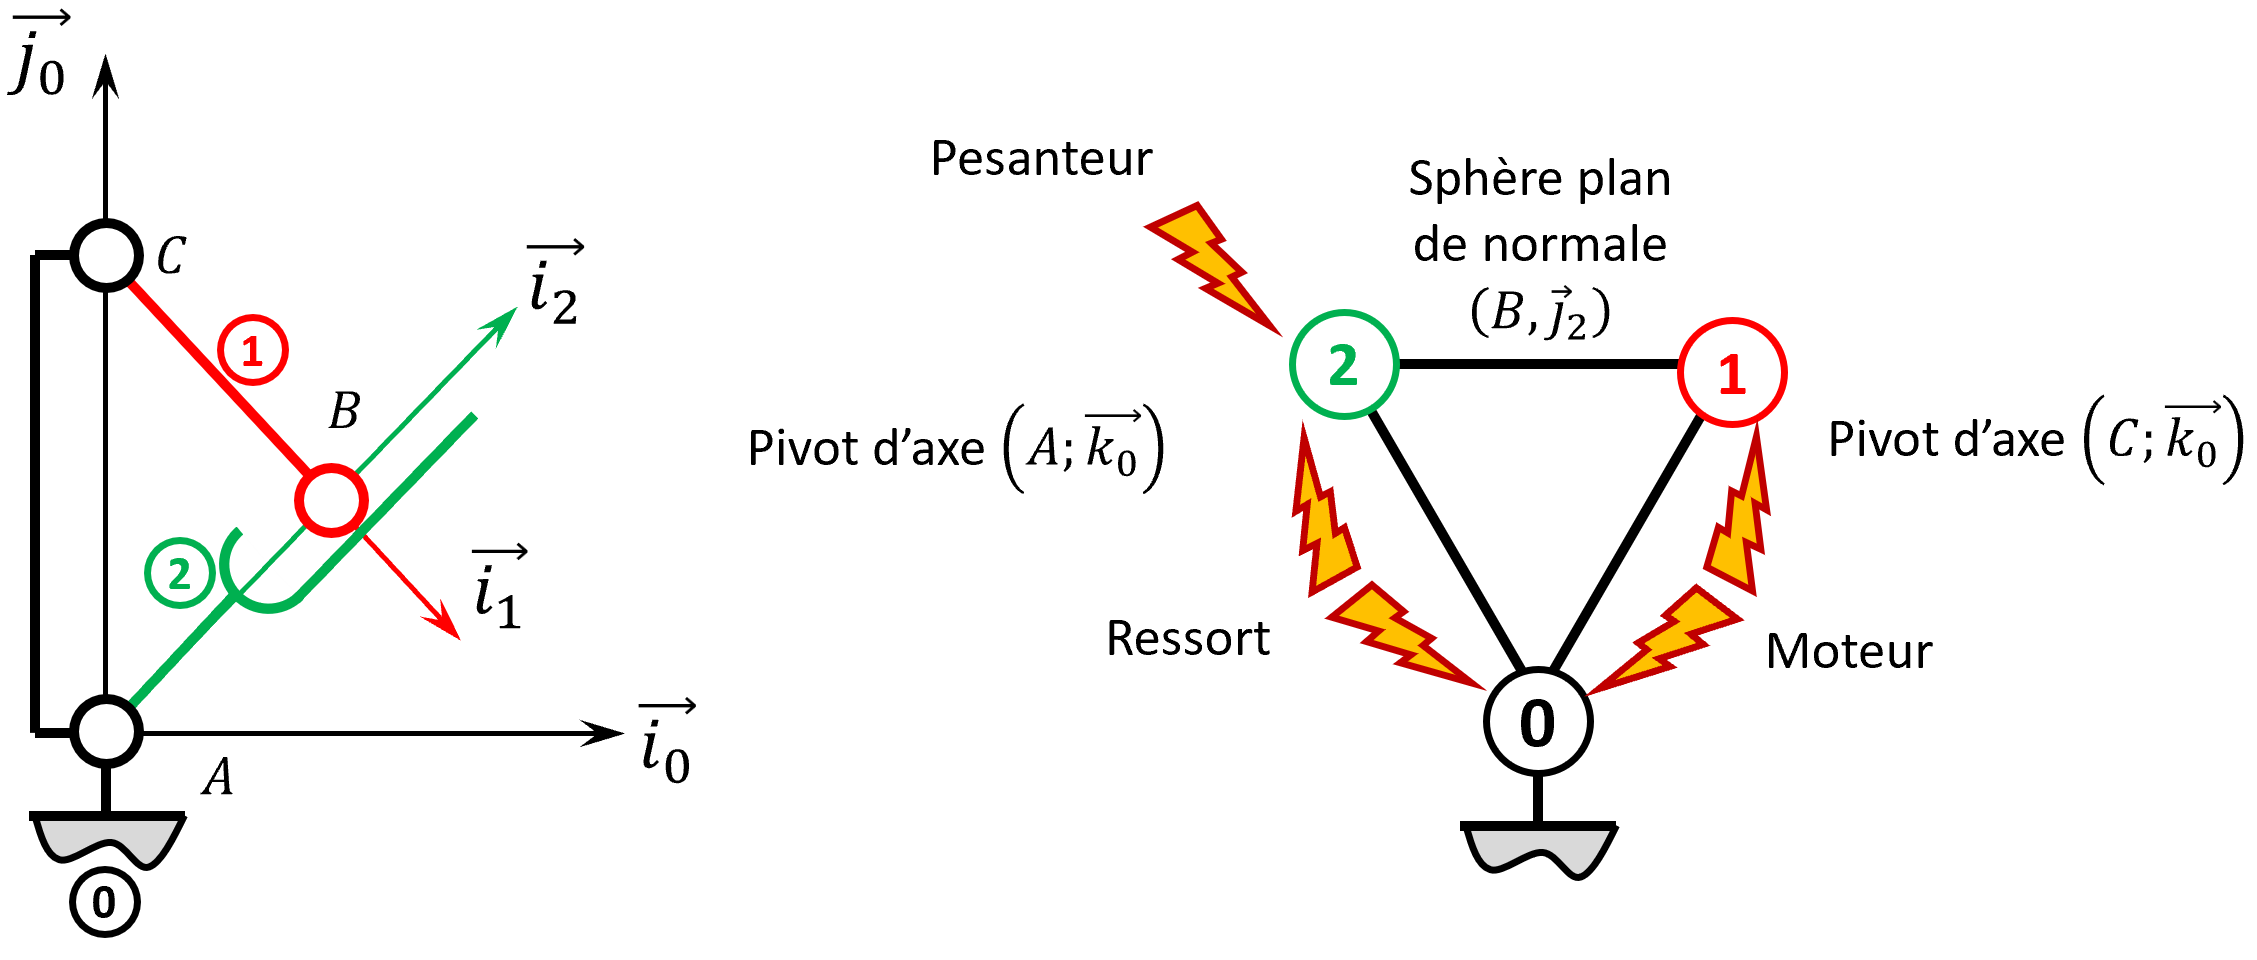
\includegraphics[width=.95\linewidth]{pfs_strategie_sympact_01}
%\end{center}
	\begin{reponses}
	\bonne{Ponctuelle}
	\bonne{Sphère plan}
	\mauvaise{Linéaire annulaire}
	\mauvaise{Sphère cylindre}
	\mauvaise{Linéaire rectiligne}
	\mauvaise{Cylindre plan}
	\mauvaise{Rotule}
	\mauvaise{Sphérique}
	\mauvaise{Rotule à doigt}
	\mauvaise{Pivot glissant}
	\mauvaise{Pivot}
	\mauvaise{Glissière}
	\mauvaise{Hélicoïdale}
	\mauvaise{Encastrement}
	\mauvaise{d'axe}
	\bonne{de normale}
	\mauvaise{de direction}
	\mauvaise{de centre}
	\mauvaise{$O$}
	\mauvaise{$\overrightarrow{x}$}
	\bonne{$\overrightarrow{y}$}
          \mauvaise{$\overrightarrow{z}$}
	\end{reponses}
\end{questionmult}
\\}


\element{liaisons statique}{
\begin{questionmult}{liaisonstat 03}
Soit le torseur des actions mécaniques suivant : 
$\torseurl{Z_O\vz{}}{\vect{0}}{O}$.
%\begin{center}
%%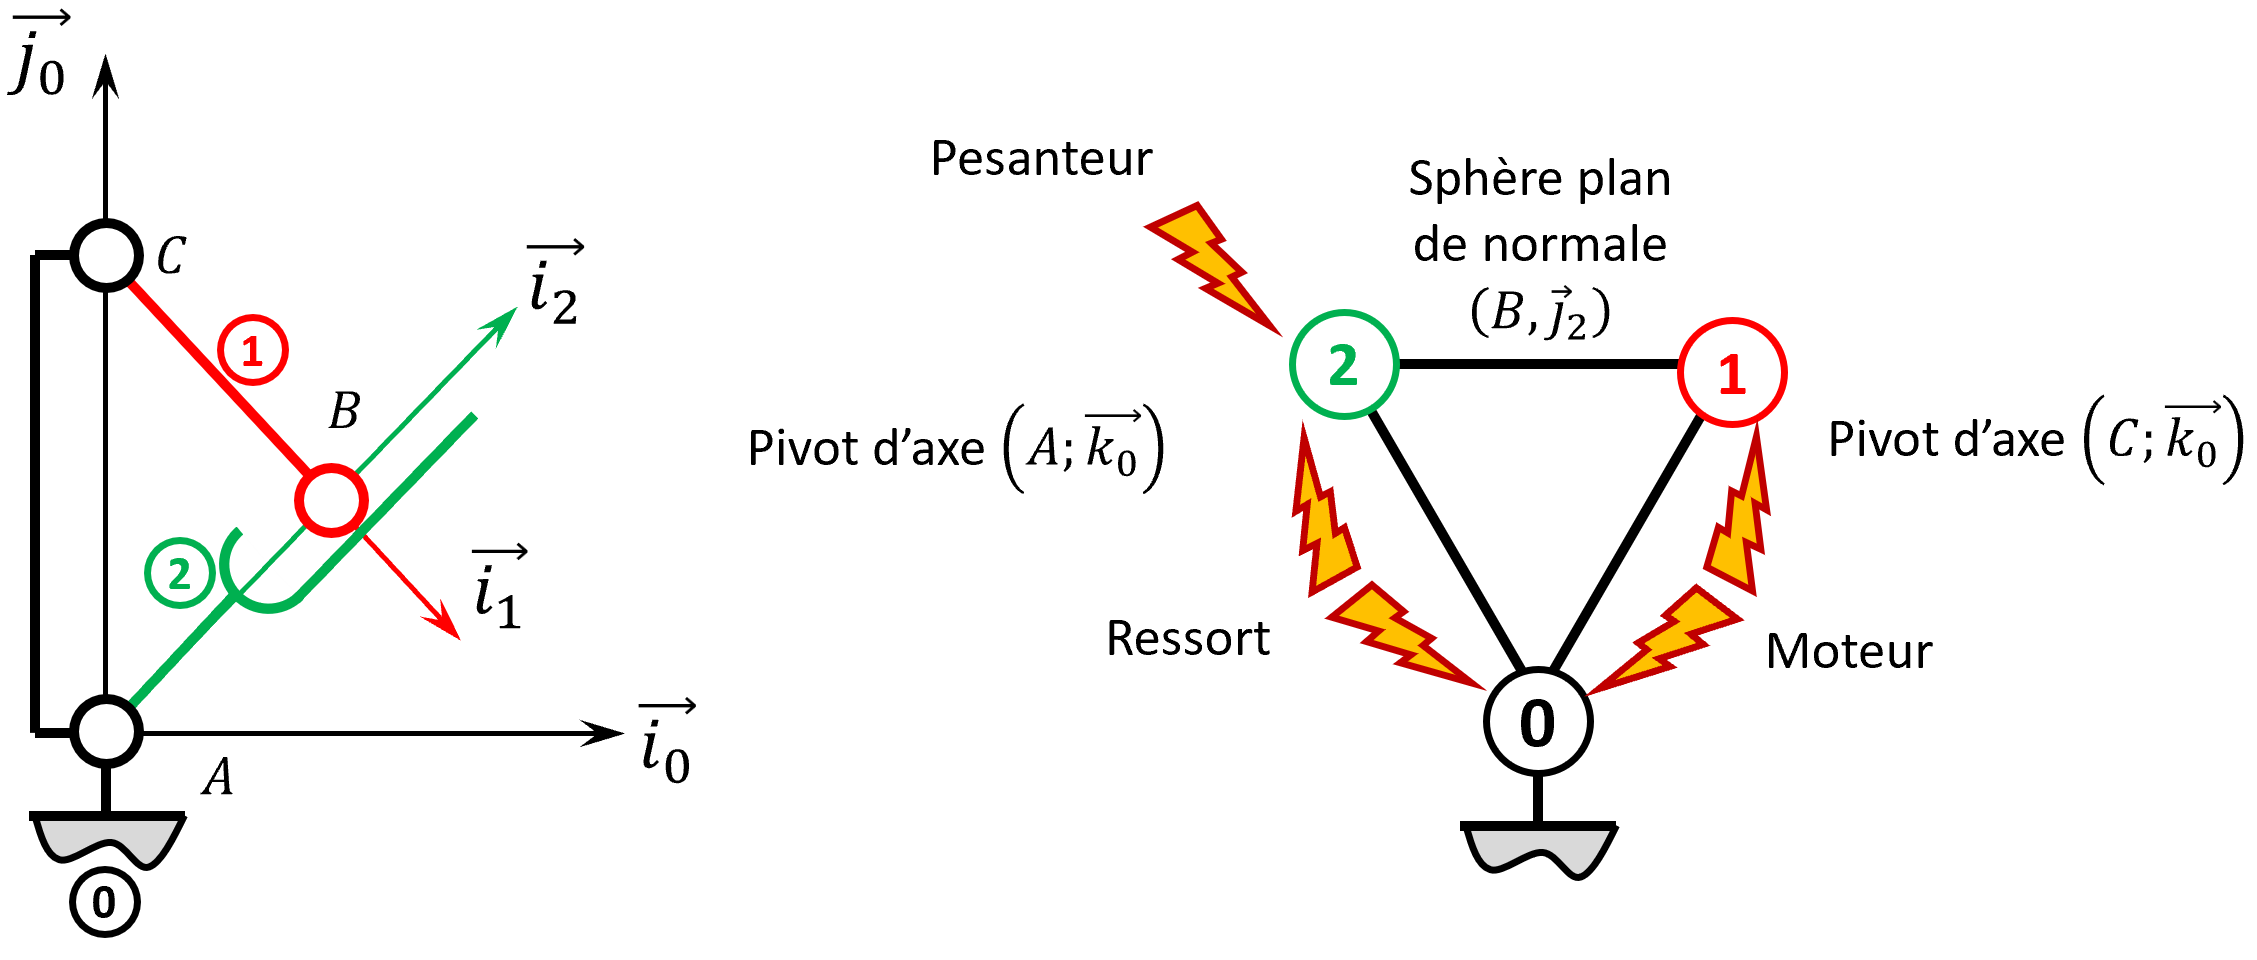
\includegraphics[width=.95\linewidth]{pfs_strategie_sympact_01}
%\end{center}
	\begin{reponses}
	\bonne{Ponctuelle}
	\bonne{Sphère plan}
	\mauvaise{Linéaire annulaire}
	\mauvaise{Sphère cylindre}
	\mauvaise{Linéaire rectiligne}
	\mauvaise{Cylindre plan}
	\mauvaise{Rotule}
	\mauvaise{Sphérique}
	\mauvaise{Rotule à doigt}
	\mauvaise{Pivot glissant}
	\mauvaise{Pivot}
	\mauvaise{Glissière}
	\mauvaise{Hélicoïdale}
	\mauvaise{Encastrement}
	\mauvaise{d'axe}
	\bonne{de normale}
	\mauvaise{de direction}
	\mauvaise{de centre}
	\mauvaise{$O$} 
	\mauvaise{$\overrightarrow{x}$}
	\mauvaise{$\overrightarrow{y}$}
          \bonne{$\overrightarrow{z}$}
	\end{reponses}
\end{questionmult}
\\}


\element{liaisons statique}{
\begin{questionmult}{liaisonstat 04}
Soit le torseur des actions mécaniques suivant : 
$\torseurl{X_O\vx{}+Y_O\vy{}}{\vect{0}}{O}$.
%\begin{center}
%%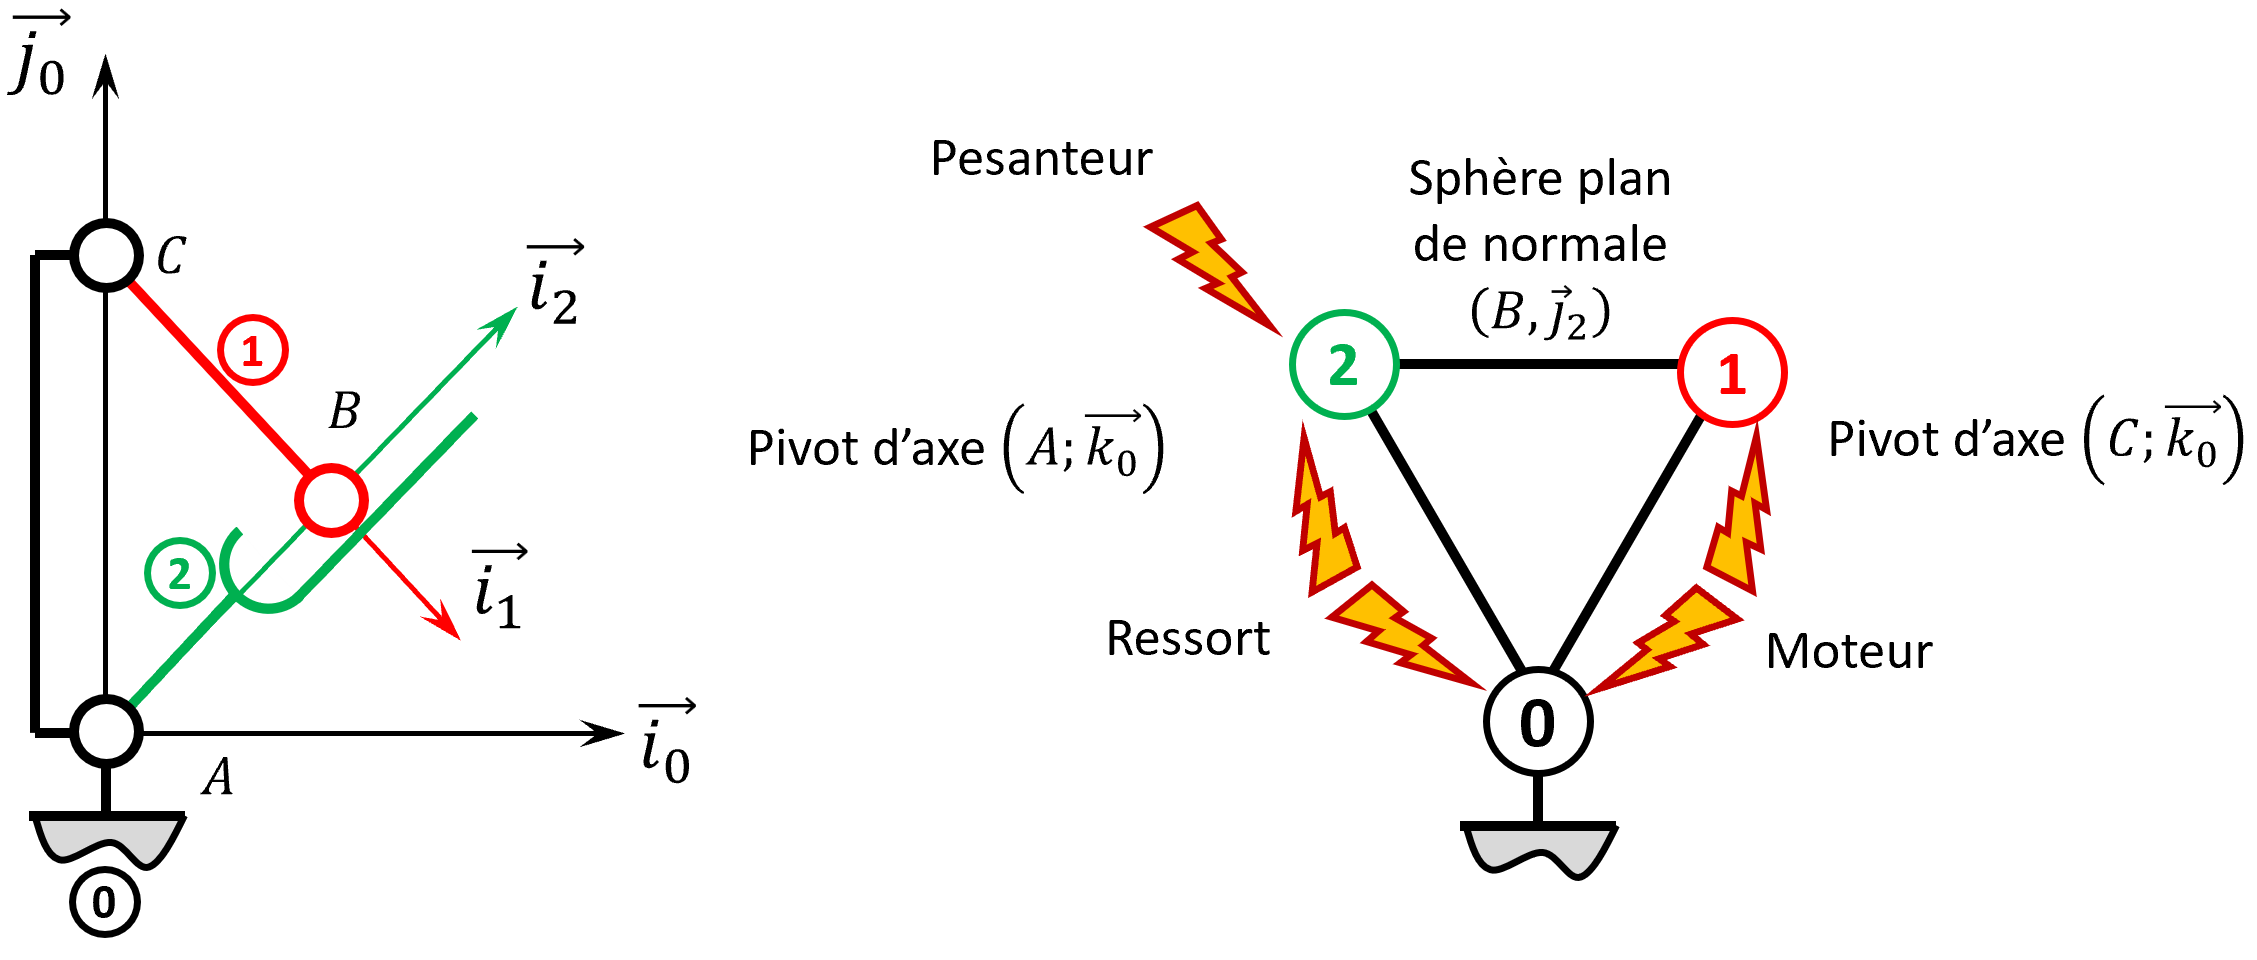
\includegraphics[width=.95\linewidth]{pfs_strategie_sympact_01}
%\end{center}
	\begin{reponses}
	\mauvaise{Ponctuelle}
	\mauvaise{Sphère plan}
	\bonne{Linéaire annulaire}
	\bonne{Sphère cylindre}
	\mauvaise{Linéaire rectiligne}
	\mauvaise{Cylindre plan}
	\mauvaise{Rotule}
	\mauvaise{Sphérique}
	\mauvaise{Rotule à doigt}
	\mauvaise{Pivot glissant}
	\mauvaise{Pivot}
	\mauvaise{Glissière}
	\mauvaise{Hélicoïdale}
	\mauvaise{Encastrement}
	\bonne{d'axe}
	\mauvaise{de normale}
	\mauvaise{de direction}
	\mauvaise{de centre}
	\bonne{$O$}
	\mauvaise{$\overrightarrow{x}$}
	\mauvaise{$\overrightarrow{y}$}
          \bonne{$\overrightarrow{z}$}
	\end{reponses}
\end{questionmult}
\\}


\element{liaisons statique}{
\begin{questionmult}{liaisonstat 05}
Soit le torseur des actions mécaniques suivant : 
$\torseurl{X_O\vx{}+Z_O\vz{}}{\vect{0}}{O}$.
%\begin{center}
%%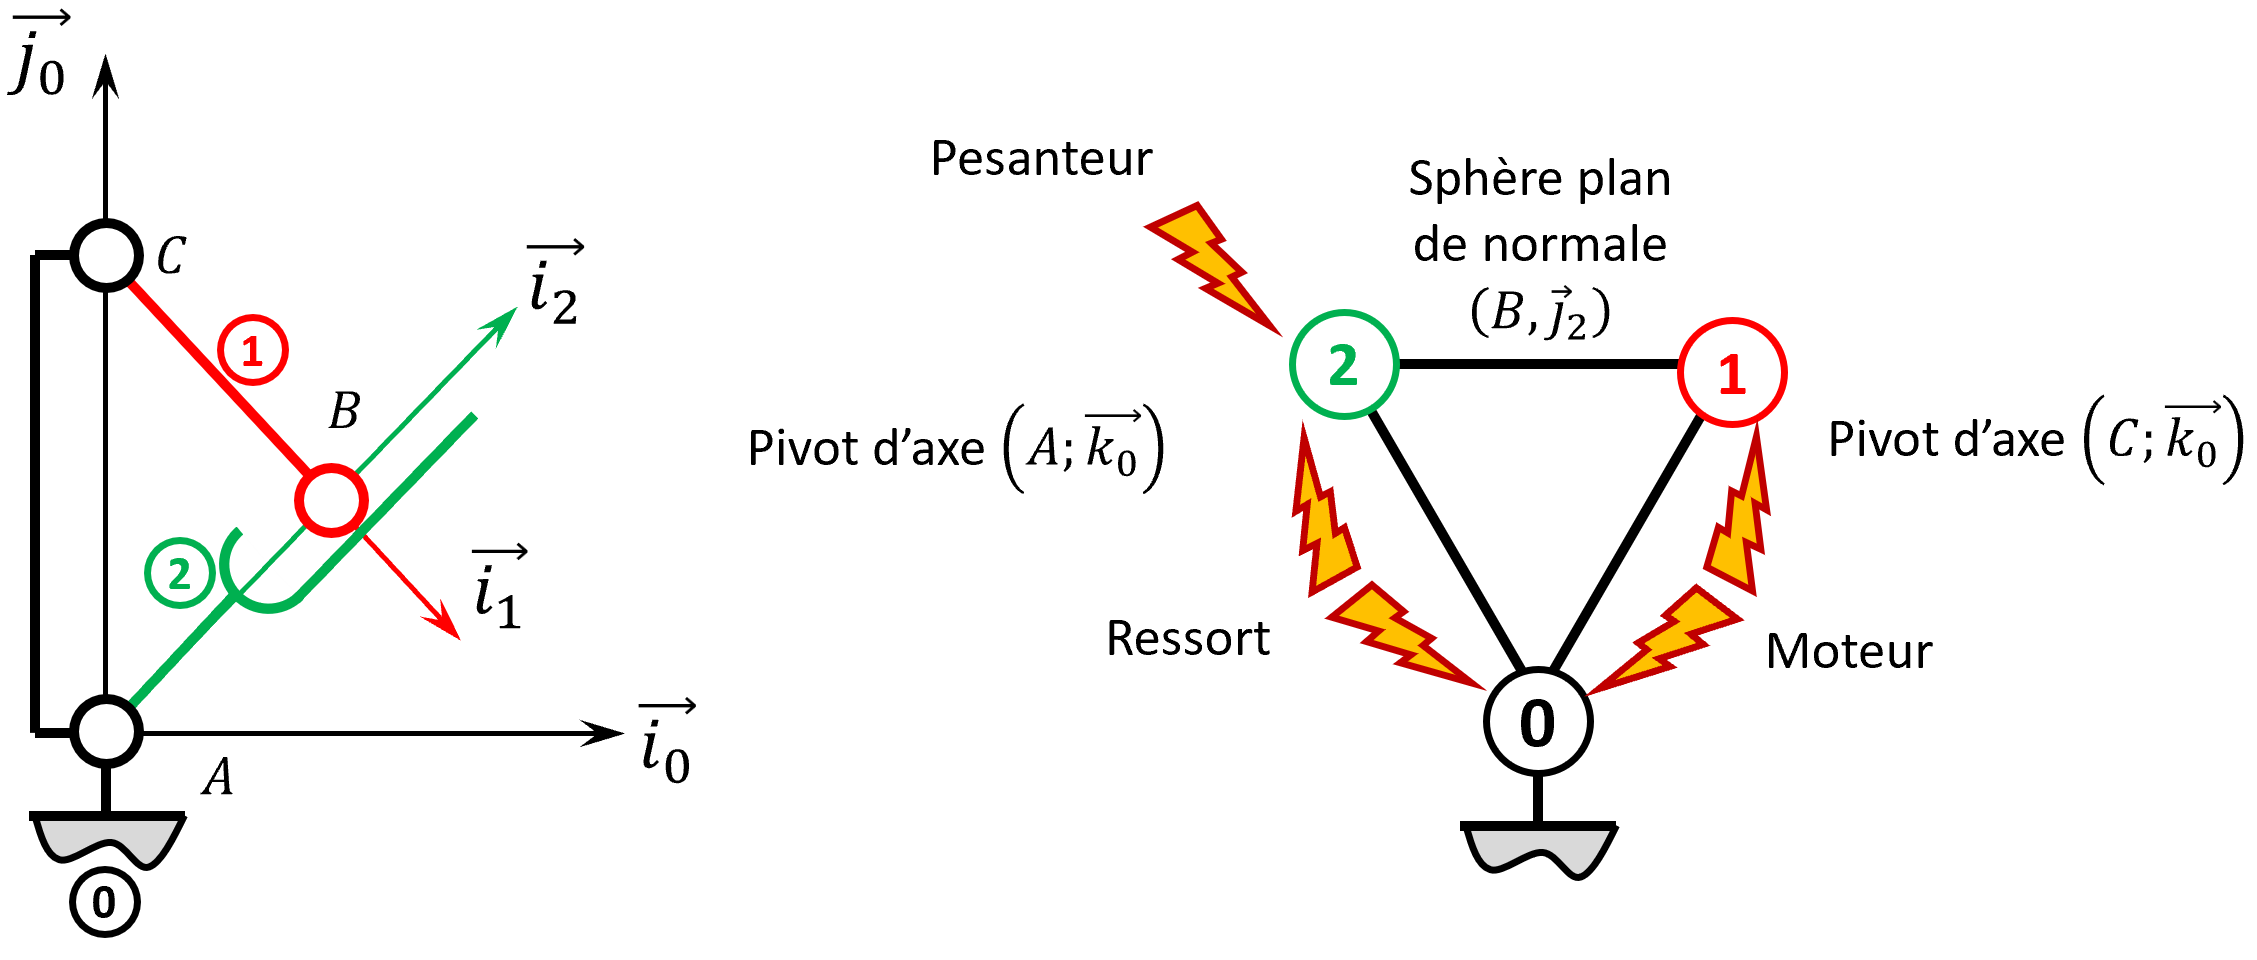
\includegraphics[width=.95\linewidth]{pfs_strategie_sympact_01}
%\end{center}
	\begin{reponses}
	\mauvaise{Ponctuelle}
	\mauvaise{Sphère plan}
	\bonne{Linéaire annulaire}
	\bonne{Sphère cylindre}
	\mauvaise{Linéaire rectiligne}
	\mauvaise{Cylindre plan}
	\mauvaise{Rotule}
	\mauvaise{Sphérique}
	\mauvaise{Rotule à doigt}
	\mauvaise{Pivot glissant}
	\mauvaise{Pivot}
	\mauvaise{Glissière}
	\mauvaise{Hélicoïdale}
	\mauvaise{Encastrement}
	\bonne{d'axe}
	\mauvaise{de normale}
	\mauvaise{de direction}
	\mauvaise{de centre}
	\bonne{$O$}
	\mauvaise{$\overrightarrow{x}$}
	\bonne{$\overrightarrow{y}$}
          \mauvaise{$\overrightarrow{z}$}
	\end{reponses}
\end{questionmult}
\\}

\element{liaisons statique}{
\begin{questionmult}{liaisonstat 06}
Soit le torseur des actions mécaniques suivant : 
$\torseurl{Y_O\vy{}+Z_O\vz{}}{\vect{0}}{O}$.
%\begin{center}
%%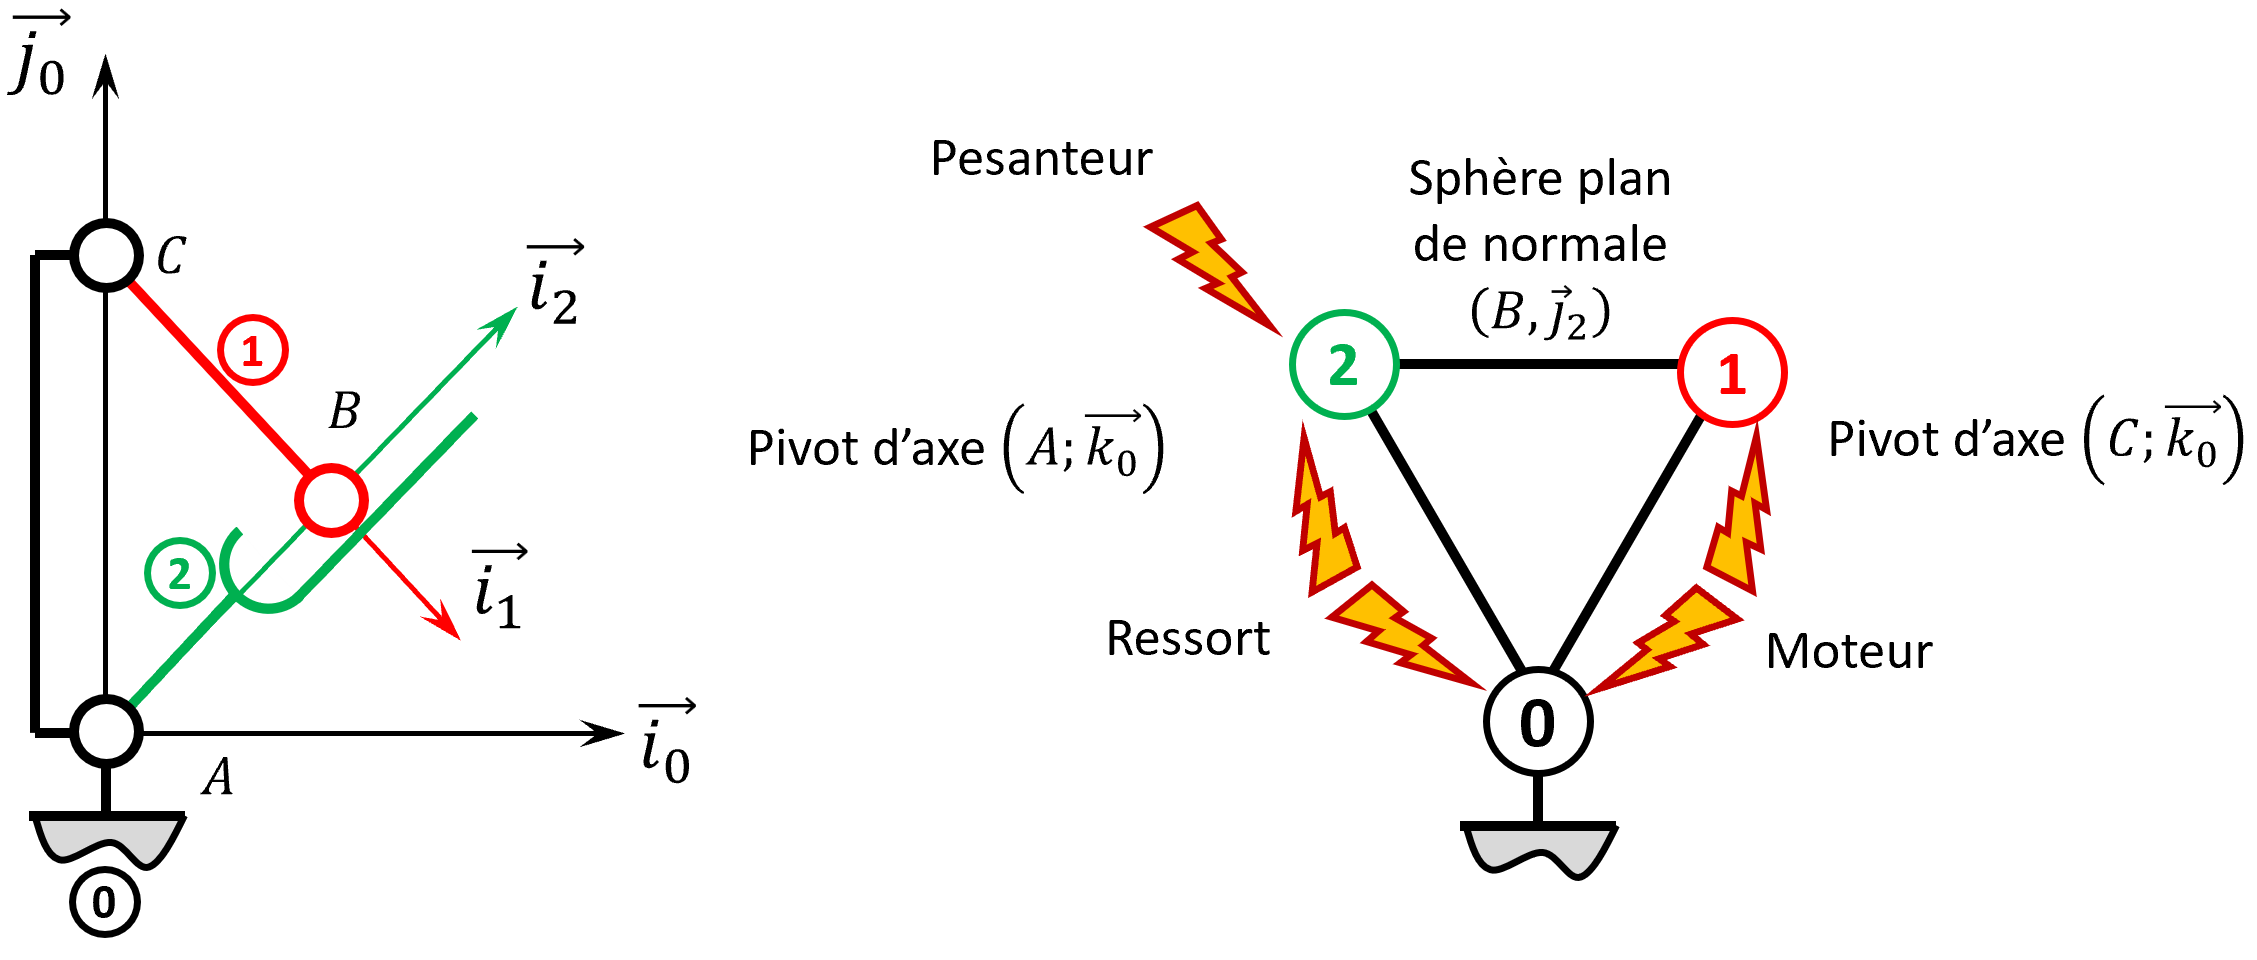
\includegraphics[width=.95\linewidth]{pfs_strategie_sympact_01}
%\end{center}
	\begin{reponses}
	\mauvaise{Ponctuelle}
	\mauvaise{Sphère plan}
	\bonne{Linéaire annulaire}
	\bonne{Sphère cylindre}
	\mauvaise{Linéaire rectiligne}
	\mauvaise{Cylindre plan}
	\mauvaise{Rotule}
	\mauvaise{Sphérique}
	\mauvaise{Rotule à doigt}
	\mauvaise{Pivot glissant}
	\mauvaise{Pivot}
	\mauvaise{Glissière}
	\mauvaise{Hélicoïdale}
	\mauvaise{Encastrement}
	\bonne{d'axe}
	\mauvaise{de normale}
	\mauvaise{de direction}
	\mauvaise{de centre}
	\bonne {$O$}
	\bonne{$\overrightarrow{x}$}
	\mauvaise{$\overrightarrow{y}$}
          \mauvaise{$\overrightarrow{z}$}
	\end{reponses}
\end{questionmult}
\\}


\element{liaisons statique}{
\begin{questionmult}{liaisonstat 07}
Soit le torseur des actions mécaniques suivant : 
$\torseurl{X_O\vx{}}{M_O\vy{}}{O}$.
\begin{center}
%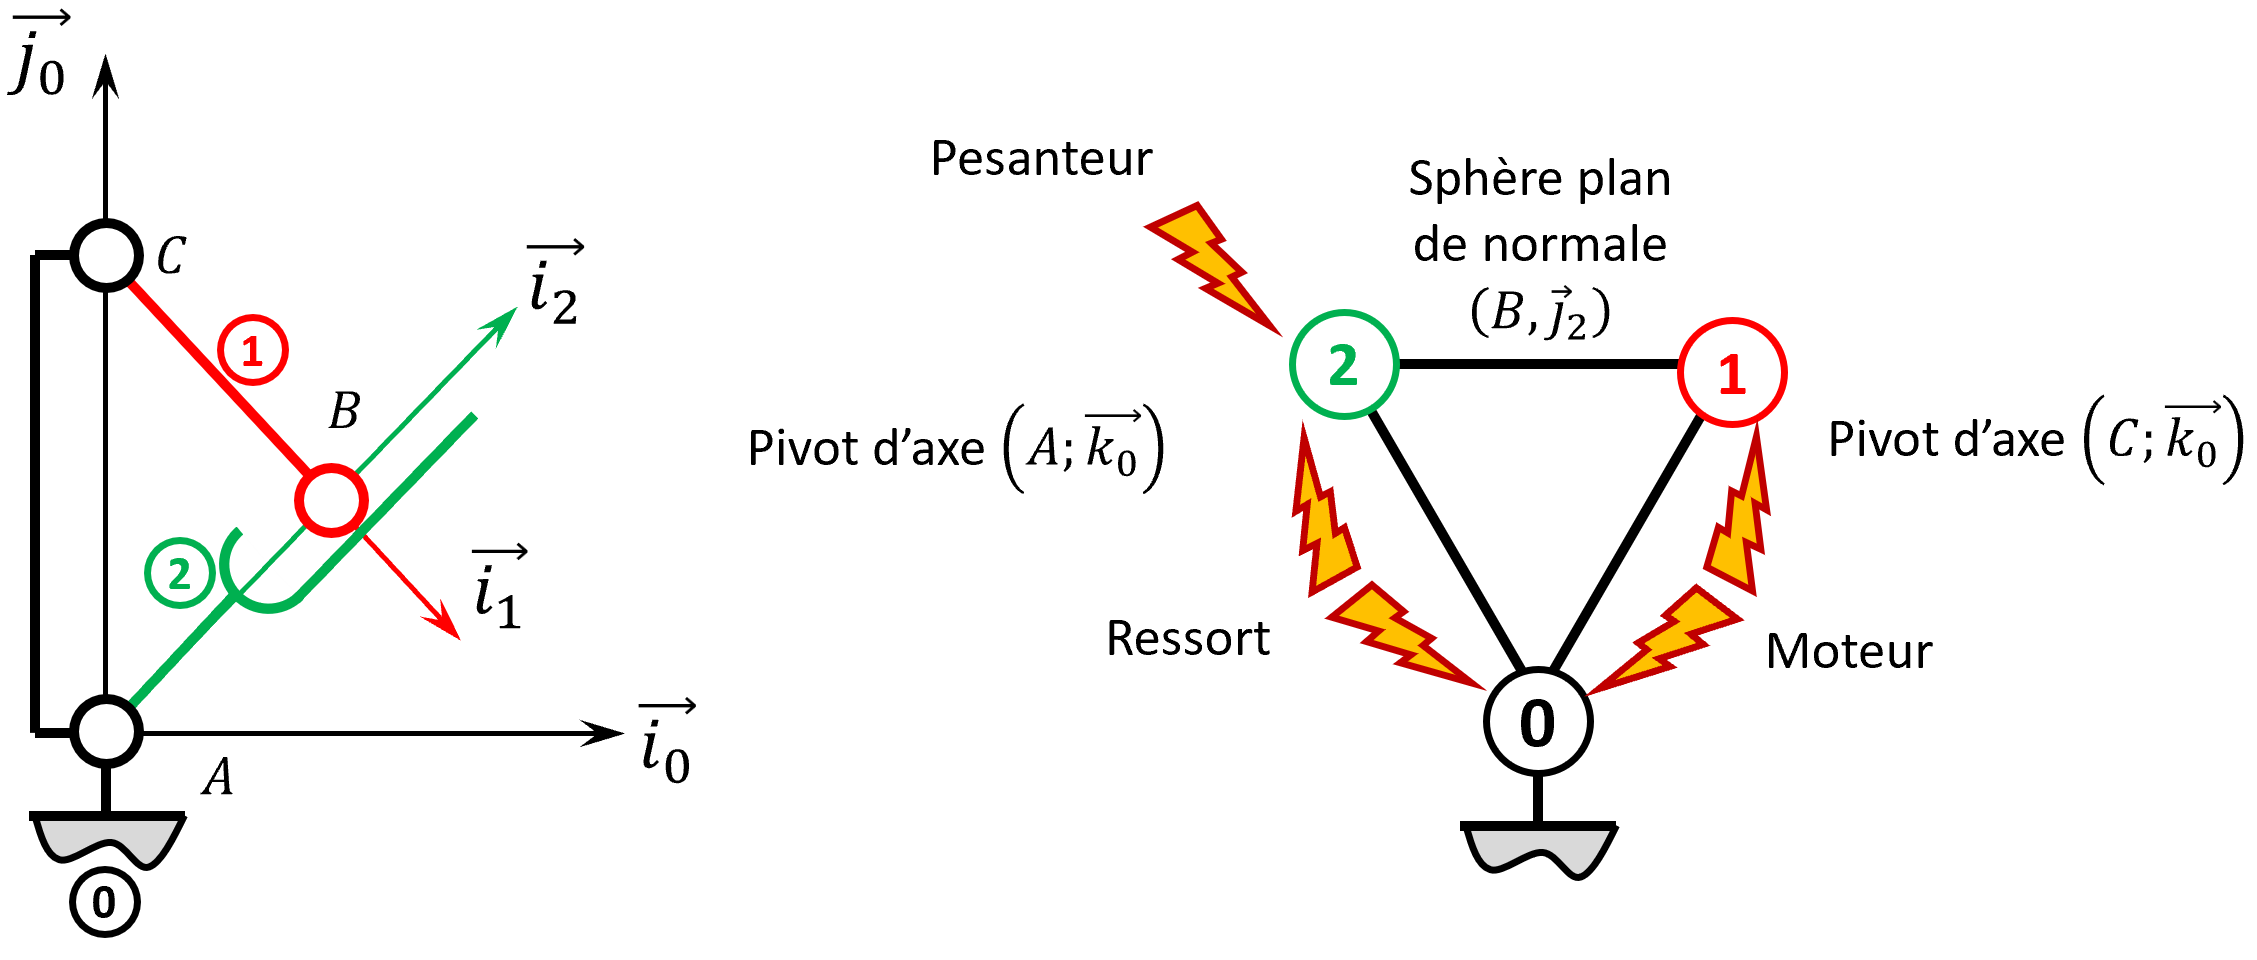
\includegraphics[width=.95\linewidth]{pfs_strategie_sympact_01}
\end{center}
	\begin{reponses}
	\mauvaise{Ponctuelle}
	\mauvaise{Sphère plan}
	\mauvaise{Linéaire annulaire}
	\mauvaise{Sphère cylindre}
	\bonne{Linéaire rectiligne}
	\bonne{Cylindre plan}
	\mauvaise{Rotule}
	\mauvaise{Sphérique}
	\mauvaise{Rotule à doigt}
	\mauvaise{Pivot glissant}
	\mauvaise{Pivot}
	\mauvaise{Glissière}
	\mauvaise{Hélicoïdale}
	\mauvaise{Encastrement}
	\bonne{d'axe}
	\bonne{de normale}
	\mauvaise{de direction}
	\mauvaise{de centre}
	\bonne {$O$}
	\bonne{$\overrightarrow{x}$}
	\mauvaise{$\overrightarrow{y}$}
          \bonne{$\overrightarrow{z}$}
	\end{reponses}
\end{questionmult}
\\}


\element{liaisons statique}{
\begin{questionmult}{liaisonstat 08}
Soit le torseur des actions mécaniques suivant : 
$\torseurl{X_O\vx{}}{N_O\vz{}}{O}$.
%\begin{center}
%%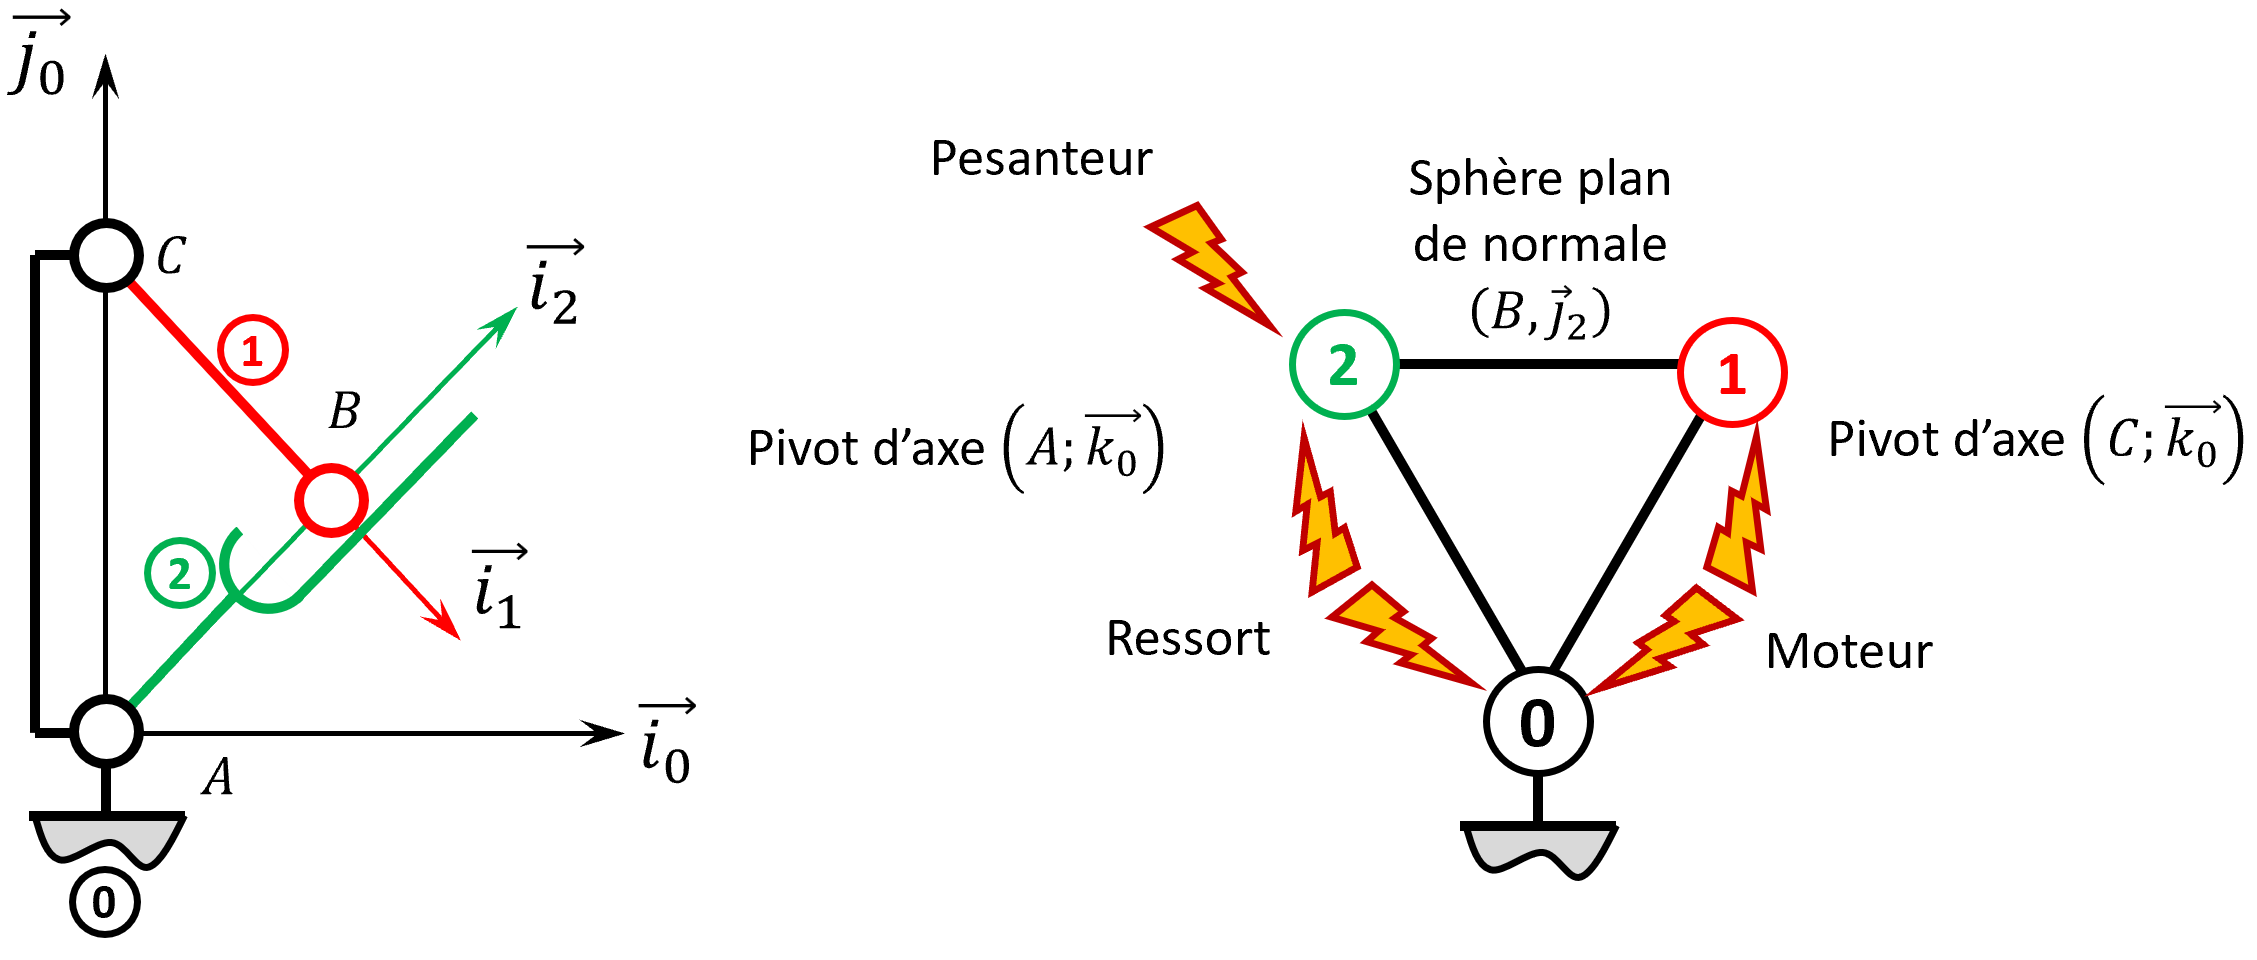
\includegraphics[width=.95\linewidth]{pfs_strategie_sympact_01}
%\end{center}
	\begin{reponses}
	\mauvaise{Ponctuelle}
	\mauvaise{Sphère plan}
	\mauvaise{Linéaire annulaire}
	\mauvaise{Sphère cylindre}
	\bonne{Linéaire rectiligne}
	\bonne{Cylindre plan}
	\mauvaise{Rotule}
	\mauvaise{Sphérique}
	\mauvaise{Rotule à doigt}
	\mauvaise{Pivot glissant}
	\mauvaise{Pivot}
	\mauvaise{Glissière}
	\mauvaise{Hélicoïdale}
	\mauvaise{Encastrement}
	\bonne{d'axe}
	\bonne{de normale}
	\mauvaise{de direction}
	\mauvaise{de centre}
	\bonne $O$
	\bonne{$\overrightarrow{x}$}
	\bonne{$\overrightarrow{y}$}
          \mauvaise{$\overrightarrow{z}$}
	\end{reponses}
\end{questionmult}
\\}


\element{liaisons statique}{
\begin{questionmult}{liaisonstat 08}
Soit le torseur des actions mécaniques suivant : 
$\torseurl{Y_O\vy{}}{N_O\vz{}}{O}$.
%\begin{center}
%%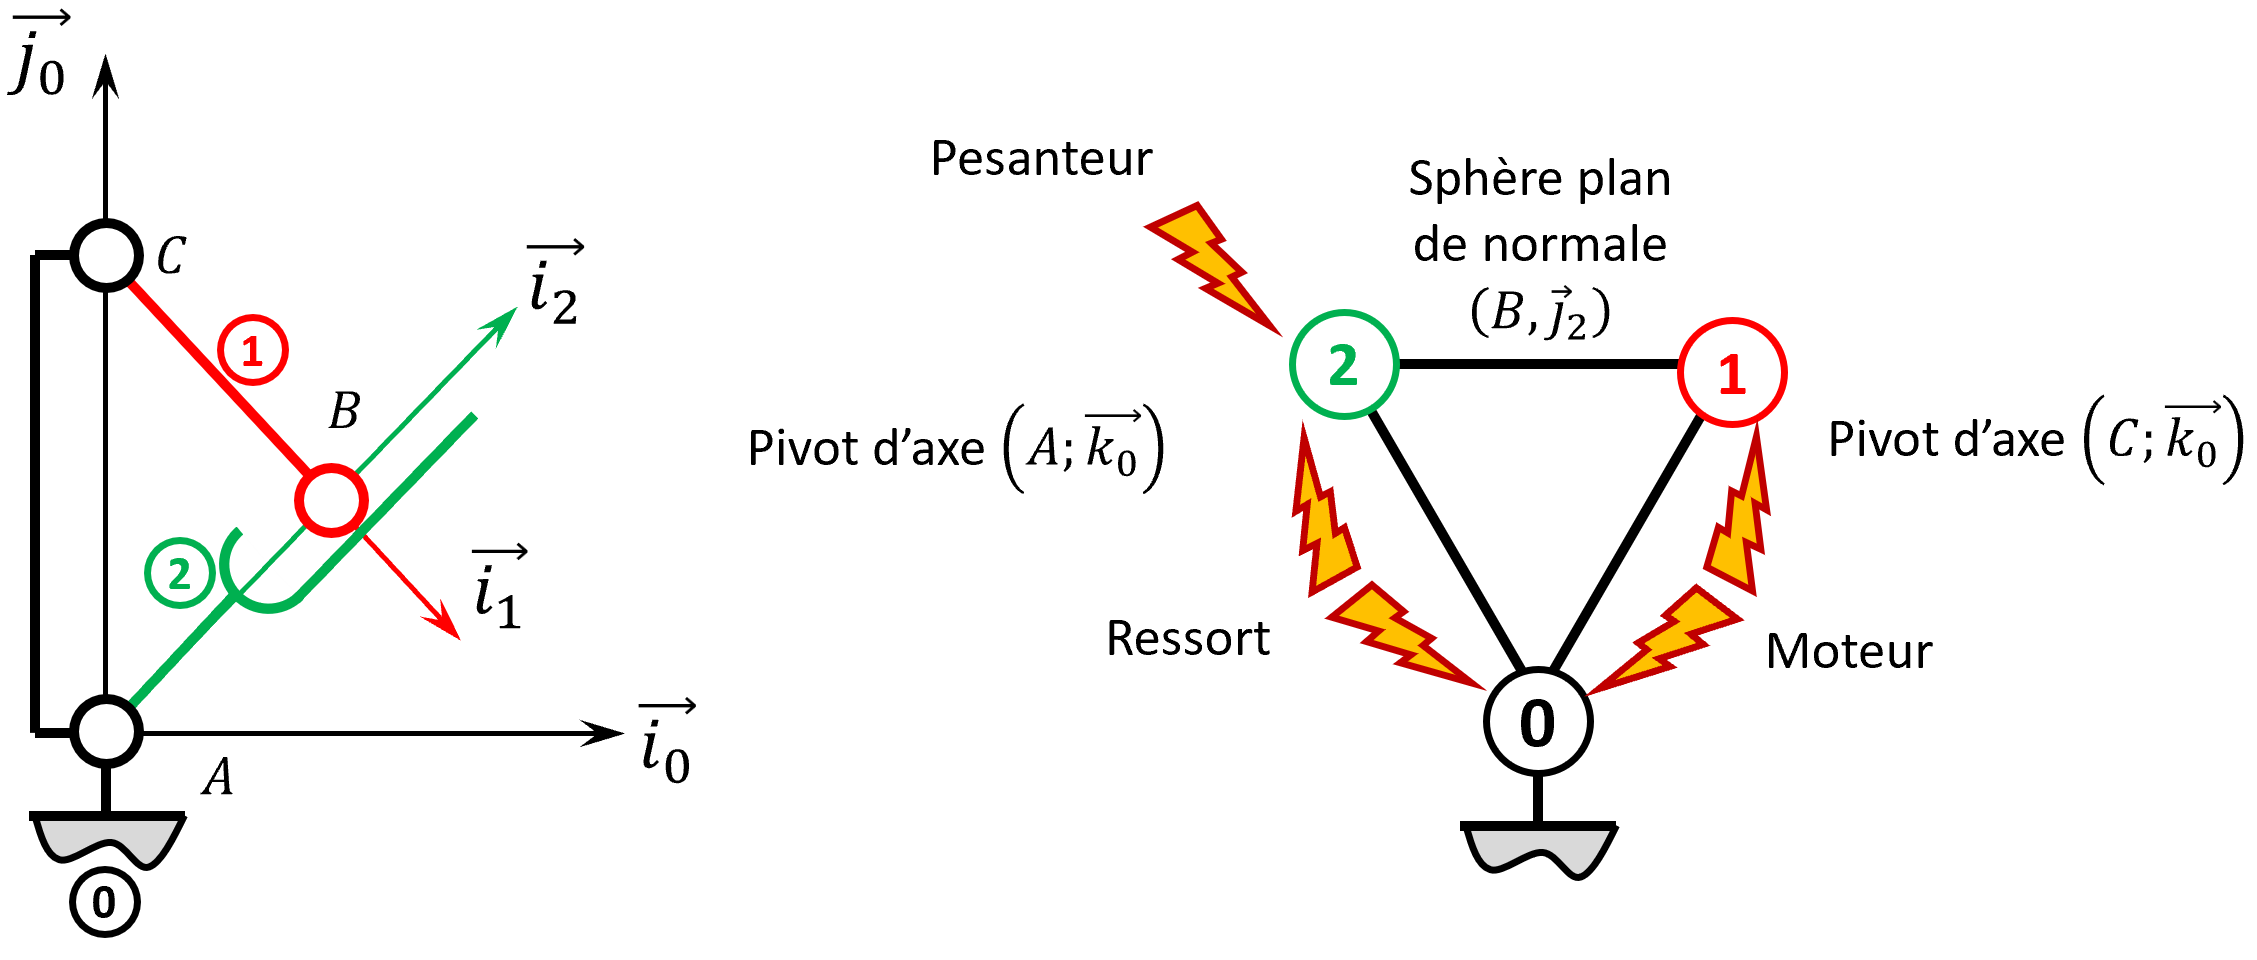
\includegraphics[width=.95\linewidth]{pfs_strategie_sympact_01}
%\end{center}
	\begin{reponses}
	\mauvaise{Ponctuelle}
	\mauvaise{Sphère plan}
	\mauvaise{Linéaire annulaire}
	\mauvaise{Sphère cylindre}
	\bonne{Linéaire rectiligne}
	\bonne{Cylindre plan}
	\mauvaise{Rotule}
	\mauvaise{Sphérique}
	\mauvaise{Rotule à doigt}
	\mauvaise{Pivot glissant}
	\mauvaise{Pivot}
	\mauvaise{Glissière}
	\mauvaise{Hélicoïdale}
	\mauvaise{Encastrement}
	\bonne{d'axe}
	\bonne{de normale}
	\mauvaise{de direction}
	\mauvaise{de centre}
	\bonne $O$
	\bonne{$\overrightarrow{x}$}
	\bonne{$\overrightarrow{y}$}
          \mauvaise{$\overrightarrow{z}$}
	\end{reponses}
\end{questionmult}
\\}


\element{liaisons statique}{
\begin{questionmult}{liaisonstat 09}
Soit le torseur des actions mécaniques suivant : 
$\torseurl{Y_O\vy{}}{L_O\vx{}}{O}$.
%\begin{center}
%%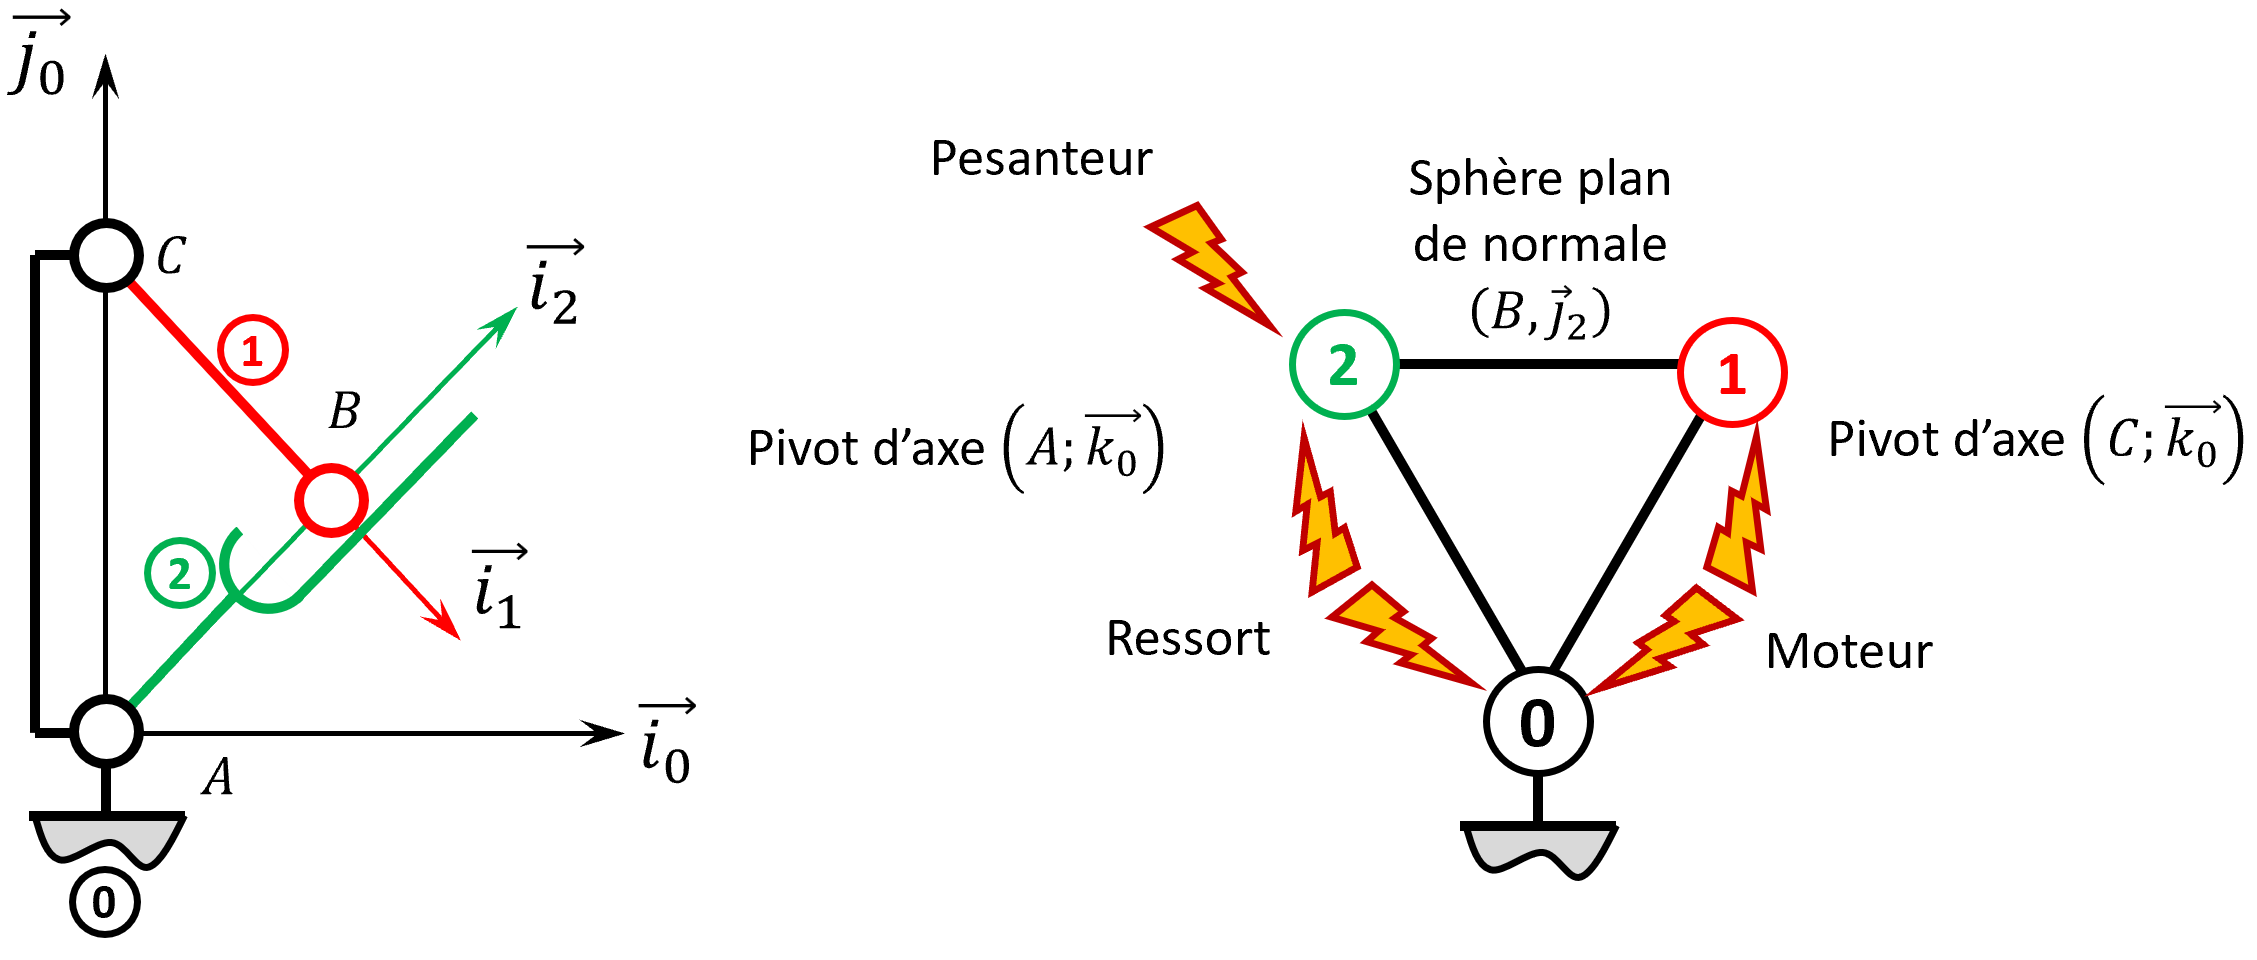
\includegraphics[width=.95\linewidth]{pfs_strategie_sympact_01}
%\end{center}
	\begin{reponses}
	\mauvaise{Ponctuelle}
	\mauvaise{Sphère plan}
	\mauvaise{Linéaire annulaire}
	\mauvaise{Sphère cylindre}
	\bonne{Linéaire rectiligne}
	\bonne{Cylindre plan}
	\mauvaise{Rotule}
	\mauvaise{Sphérique}
	\mauvaise{Rotule à doigt}
	\mauvaise{Pivot glissant}
	\mauvaise{Pivot}
	\mauvaise{Glissière}
	\mauvaise{Hélicoïdale}
	\mauvaise{Encastrement}
	\bonne{d'axe}
	\bonne{de normale}
	\mauvaise{de direction}
	\mauvaise{de centre}
	\bonne $O$
	\bonne{$\overrightarrow{x}$}
	\mauvaise{$\overrightarrow{y}$}
          \bonne{$\overrightarrow{z}$}
	\end{reponses}
\end{questionmult}
\\}

\element{liaisons statique}{
\begin{questionmult}{liaisonstat 10}
Soit le torseur des actions mécaniques suivant : 
$\torseurl{Z_O\vz{}}{L_O\vx{}}{O}$.
%\begin{center}
%%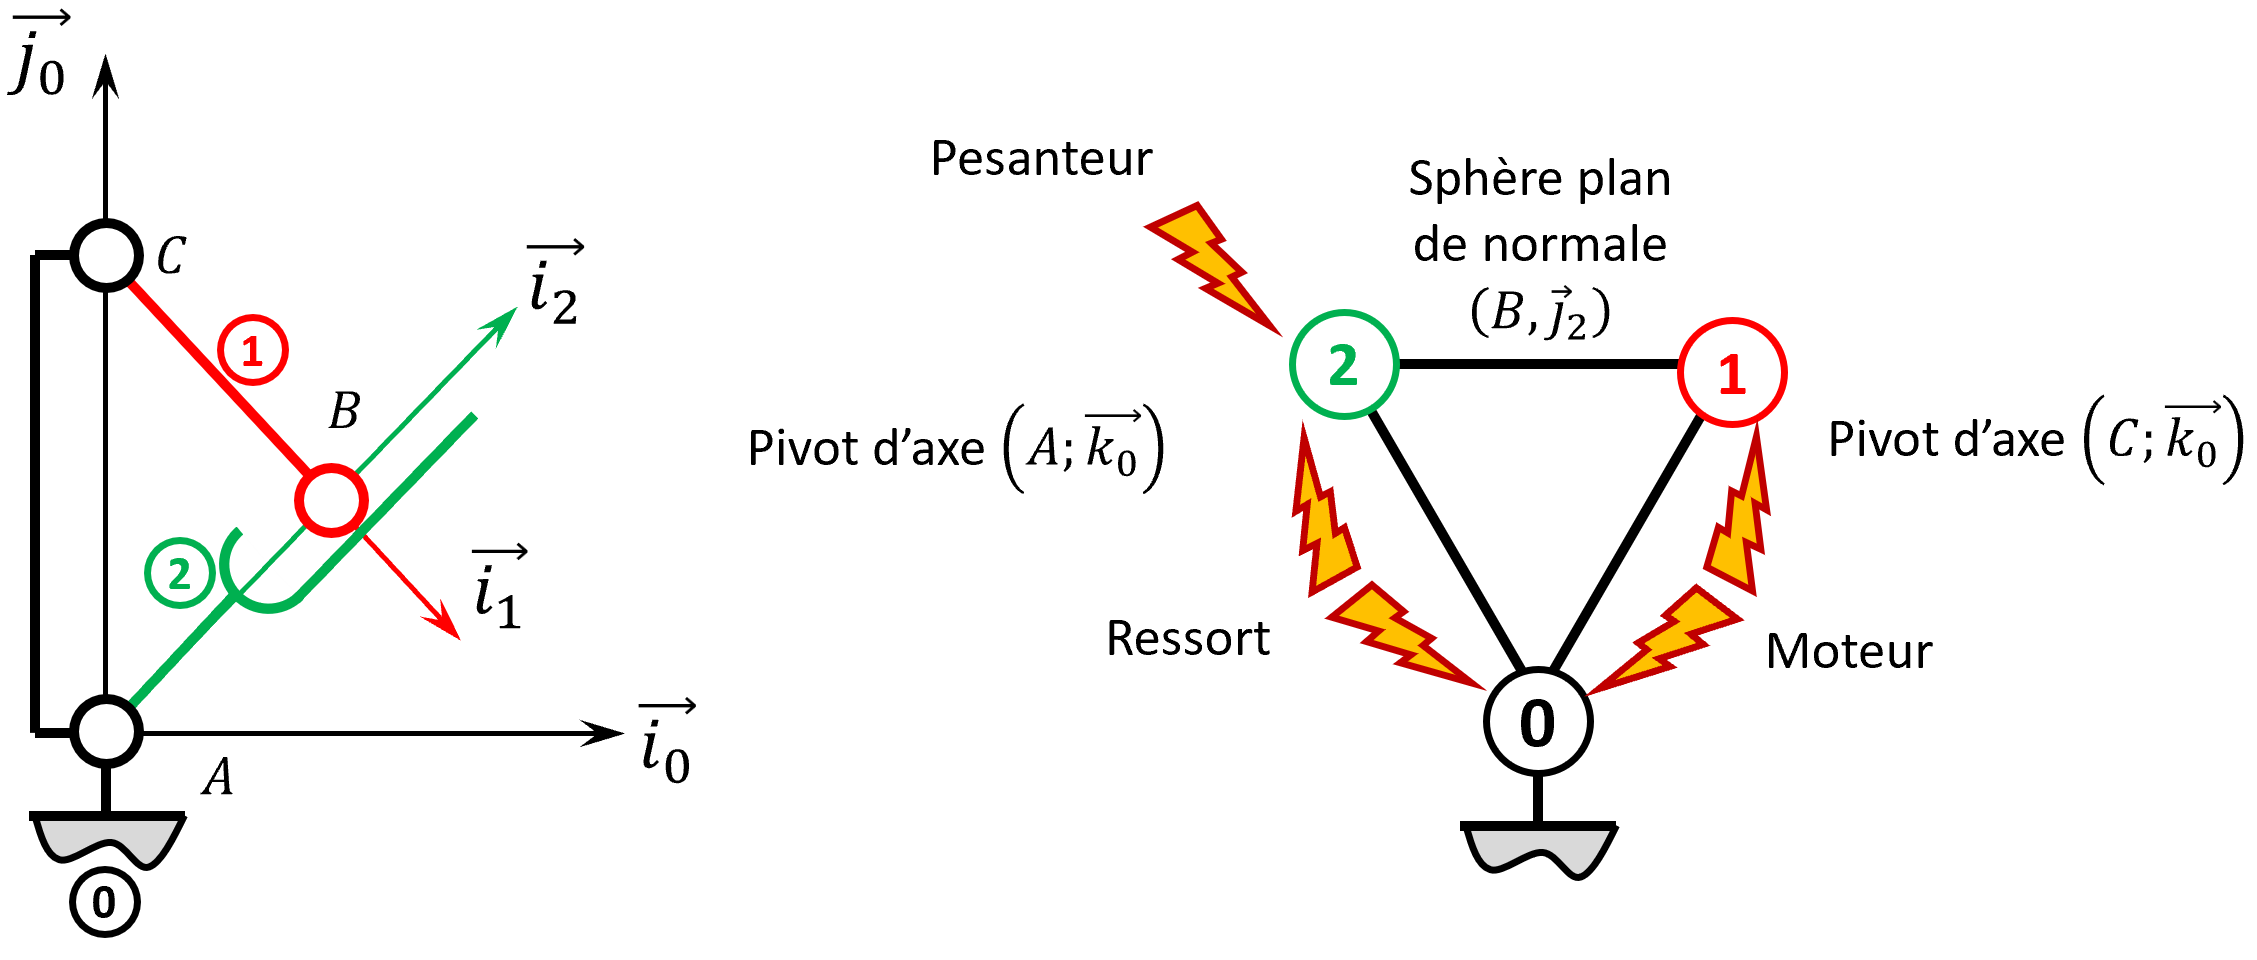
\includegraphics[width=.95\linewidth]{pfs_strategie_sympact_01}
%\end{center}
	\begin{reponses}
	\mauvaise{Ponctuelle}
	\mauvaise{Sphère plan}
	\mauvaise{Linéaire annulaire}
	\mauvaise{Sphère cylindre}
	\bonne{Linéaire rectiligne}
	\bonne{Cylindre plan}
	\mauvaise{Rotule}
	\mauvaise{Sphérique}
	\mauvaise{Rotule à doigt}
	\mauvaise{Pivot glissant}
	\mauvaise{Pivot}
	\mauvaise{Glissière}
	\mauvaise{Hélicoïdale}
	\mauvaise{Encastrement}
	\bonne{d'axe}
	\bonne{de normale}
	\mauvaise{de direction}
	\mauvaise{de centre}
	\bonne $O$
	\mauvaise{$\overrightarrow{x}$}
	\bonne{$\overrightarrow{y}$}
          \bonne{$\overrightarrow{z}$}
	\end{reponses}
\end{questionmult}
\\}

\element{liaisons statique}{
\begin{questionmult}{liaisonstat 11}
Soit le torseur des actions mécaniques suivant : 
$\torseurl{Z_O\vz{}}{M_O\vy{}}{O}$.
%\begin{center}
%%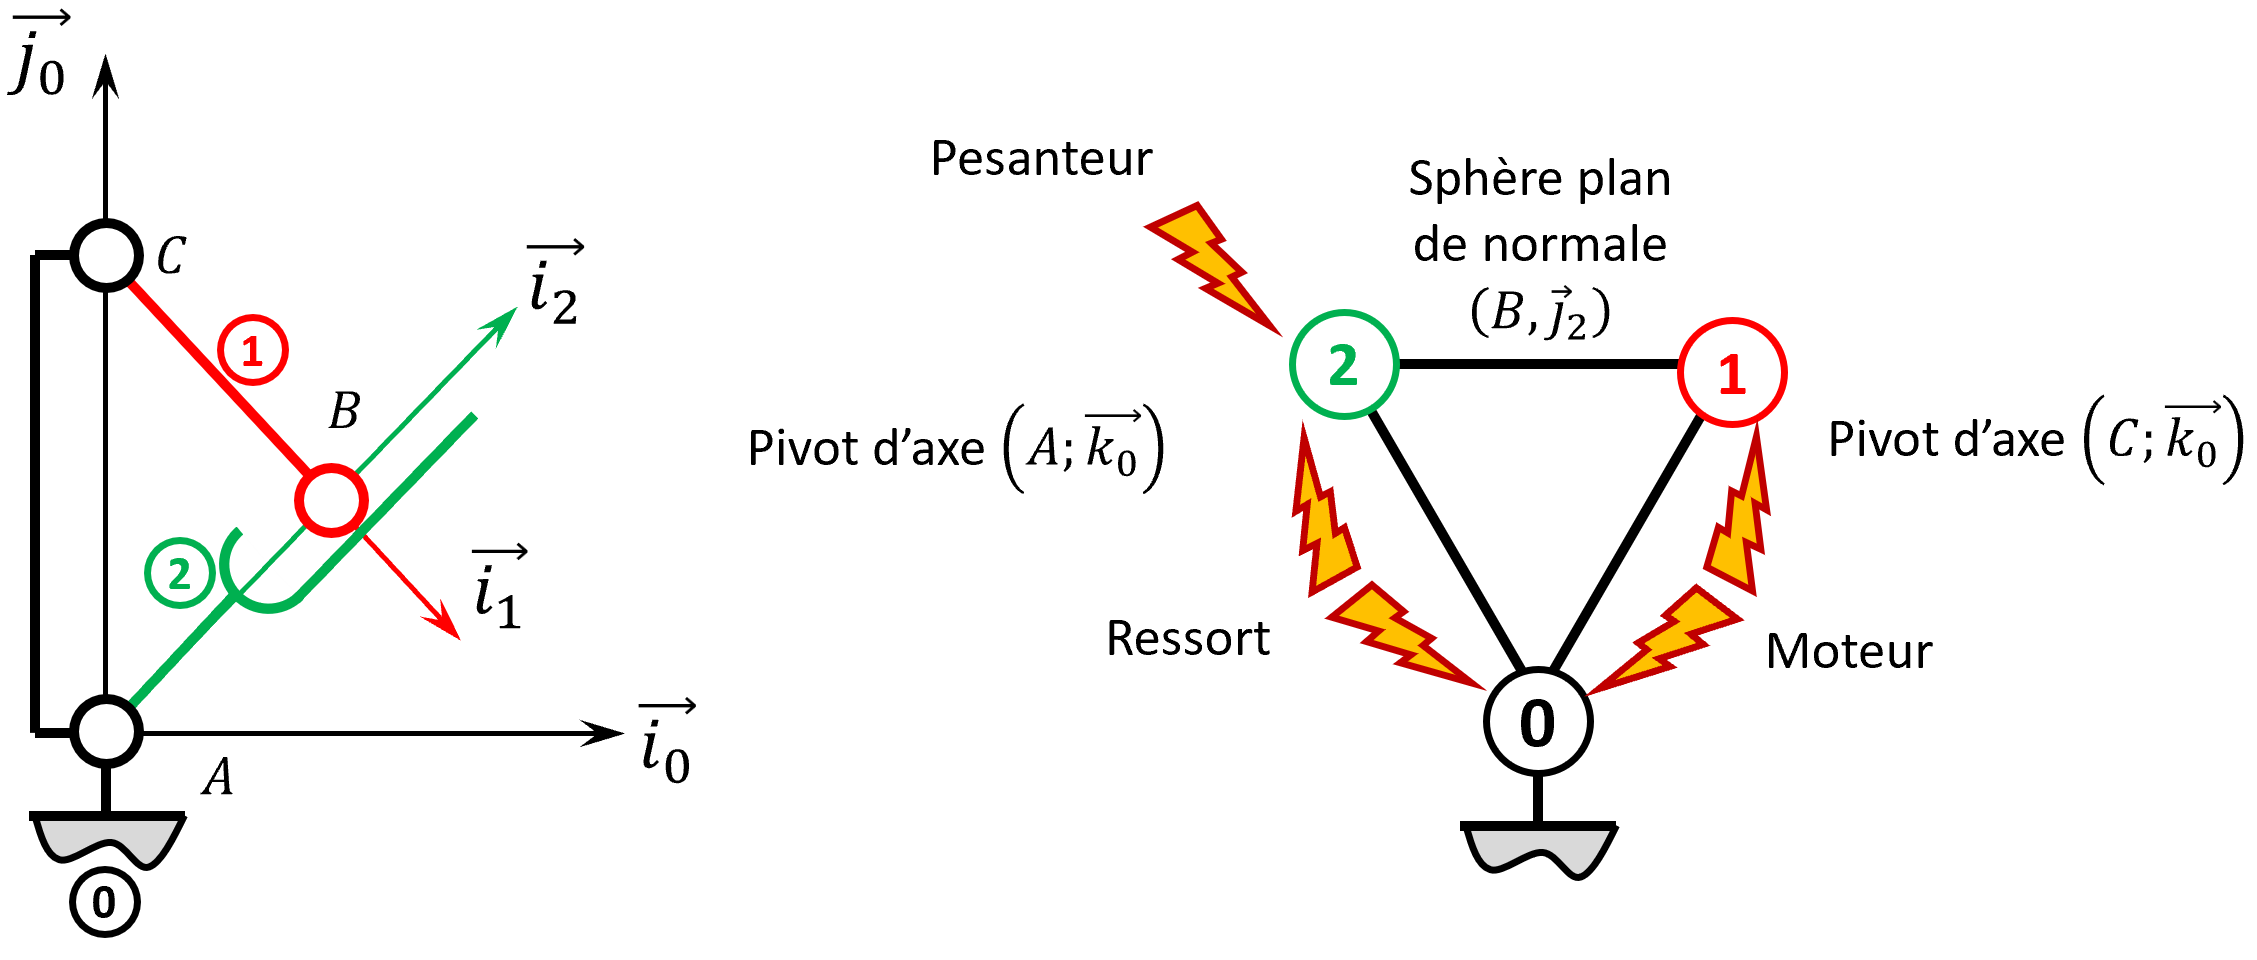
\includegraphics[width=.95\linewidth]{pfs_strategie_sympact_01}
%\end{center}
	\begin{reponses}
	\mauvaise{Ponctuelle}
	\mauvaise{Sphère plan}
	\mauvaise{Linéaire annulaire}
	\mauvaise{Sphère cylindre}
	\bonne{Linéaire rectiligne}
	\bonne{Cylindre plan}
	\mauvaise{Rotule}
	\mauvaise{Sphérique}
	\mauvaise{Rotule à doigt}
	\mauvaise{Pivot glissant}
	\mauvaise{Pivot}
	\mauvaise{Glissière}
	\mauvaise{Hélicoïdale}
	\mauvaise{Encastrement}
	\bonne{d'axe}
	\bonne{de normale}
	\mauvaise{de direction}
	\mauvaise{de centre}
	\bonne $O$
	\bonne{$\overrightarrow{x}$}
	\mauvaise{$\overrightarrow{y}$}
          \bonne{$\overrightarrow{z}$}
	\end{reponses}
\end{questionmult}
\\}
